\chapter{Influence of the solar wind on Jupiter's current sheet structure}

\section{Introduction}

Ionization of Iogenic neutrals adds  $\sim$1 ton/s of mass to the inner magnetosphere of Jupiter, which increases the content of the corotating flux tubes \cite{Bagenal2011b}. Strong centrifugal forces in the equatorial regions of the Jovian magnetosphere stretch these flux tubes in the radial direction, which leads to the formation of a disk-like current sheet at all longitudes \cite{Khurana2004a} and distorts the magnetic field from the `dipolar' configuration. However, the Jovian current sheet is not static, and its location changes as a function of radial distance and SIII longitude due to various dynamical processes in the magnetosphere. The first such process which modifies the equatorial current sheet was discussed in Chapter 5, where we studied the implications of a thin current sheet which is unstable to the tearing instability. The resulting multiple X-line reconnection creates O-lines and flux ropes on the ion-inertial scale, which can coalesce to form large plasmoids; much like what has been seen at the terrestrial magnetopause and magnetotail \cite{AkhavanTafti2020ComparativeEvents, Eastwood2005ObservationsStudy}.

The second mechanism which perturbs the current sheet is related to the changing planetary magnetic field. Early studies of the Jovian magnetosphere, either through the detection of radio emissions \cite{Carr1969TheJupiter} or in-situ spacecraft flybys \cite{Smith1974The10}, had shown that the internal field of the planet could be better described as a dipole which is tilted with respect to the spin axis. The tilted dipole field rotates at the planetary rotation period and introduces a $\sim$10 hour periodicity in the magnetosphere. Magnetic field observations made by Pioneer 10 \cite{Smith1974The10} clearly show this 10-hour periodicity in the form of a `square-wave' signal in the radial component of the magnetic field. These findings were later confirmed by Pioneer 11 \cite{Smith1975Jupiters11}, Voyager 1 and Voyager 2 \cite{Behannon1981}, Galileo \cite{Khurana1992a, Khurana2005} and the Juno spacecraft. With the introduction of dedicated orbiters, namely Galileo and Juno, more sophisticated models of Jupiter's internal field were developed using spherical harmonics. The VIP4 model was obtained by fitting magnetic field observations from Galileo and uses fourth order harmonics \cite{Connerney1998NewFootprint}, whereas the more recent JRM09 field model \cite{Connerney2018} uses the magnetic field data obtained from Juno's close perijove passes and uses 10th order harmonics. The models show that the Jovian magnetic field is not dipolar and the higher order harmonics have a substantial contribution near the planet. Figure \ref{fig:JRM09} shows the contours of magnetic field magnitude on the 1 bar surface of Jupiter as per the JRM09 magnetic field model.

Another mechanism which temporarily modifies the structure of the current sheet is in the form of perturbations with frequencies smaller than that of the planet's rotation. One such transient perturbation relates to times when multiple current sheet crossings are observed within an interval of roughly 1 to 2 hours. This phenomena is termed as `magnetotail flapping' and is also seen to occur in the terrestrial and Kronian magnetosphere \cite{Volwerk2013ComparativeSaturn}. 

\begin{figure}
    \centering
    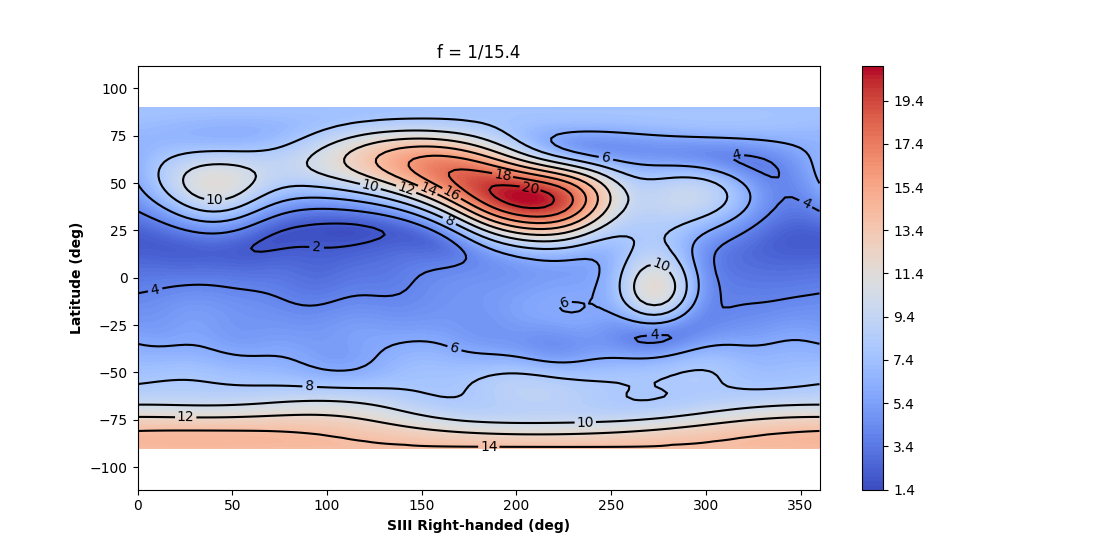
\includegraphics[width=\textwidth]{images6/JRM09_Bmag.png}
    \caption{Contours of the magnetic field strength (in Gauss) on a representative flattened ellipsoid surface of Jupiter as per the JRM09 magnetic field model. The System III longitude system is a left-handed planetocentric coordinate system often used in studies of the Jovian system. In this system, the planetary magnetic field is fixed, and the system rotates about Jupiter's spin axis at its rotation period. 
    \protect\cite{Connerney2018}.}
    \label{fig:JRM09}
\end{figure}

\begin{figure}
    \centering
    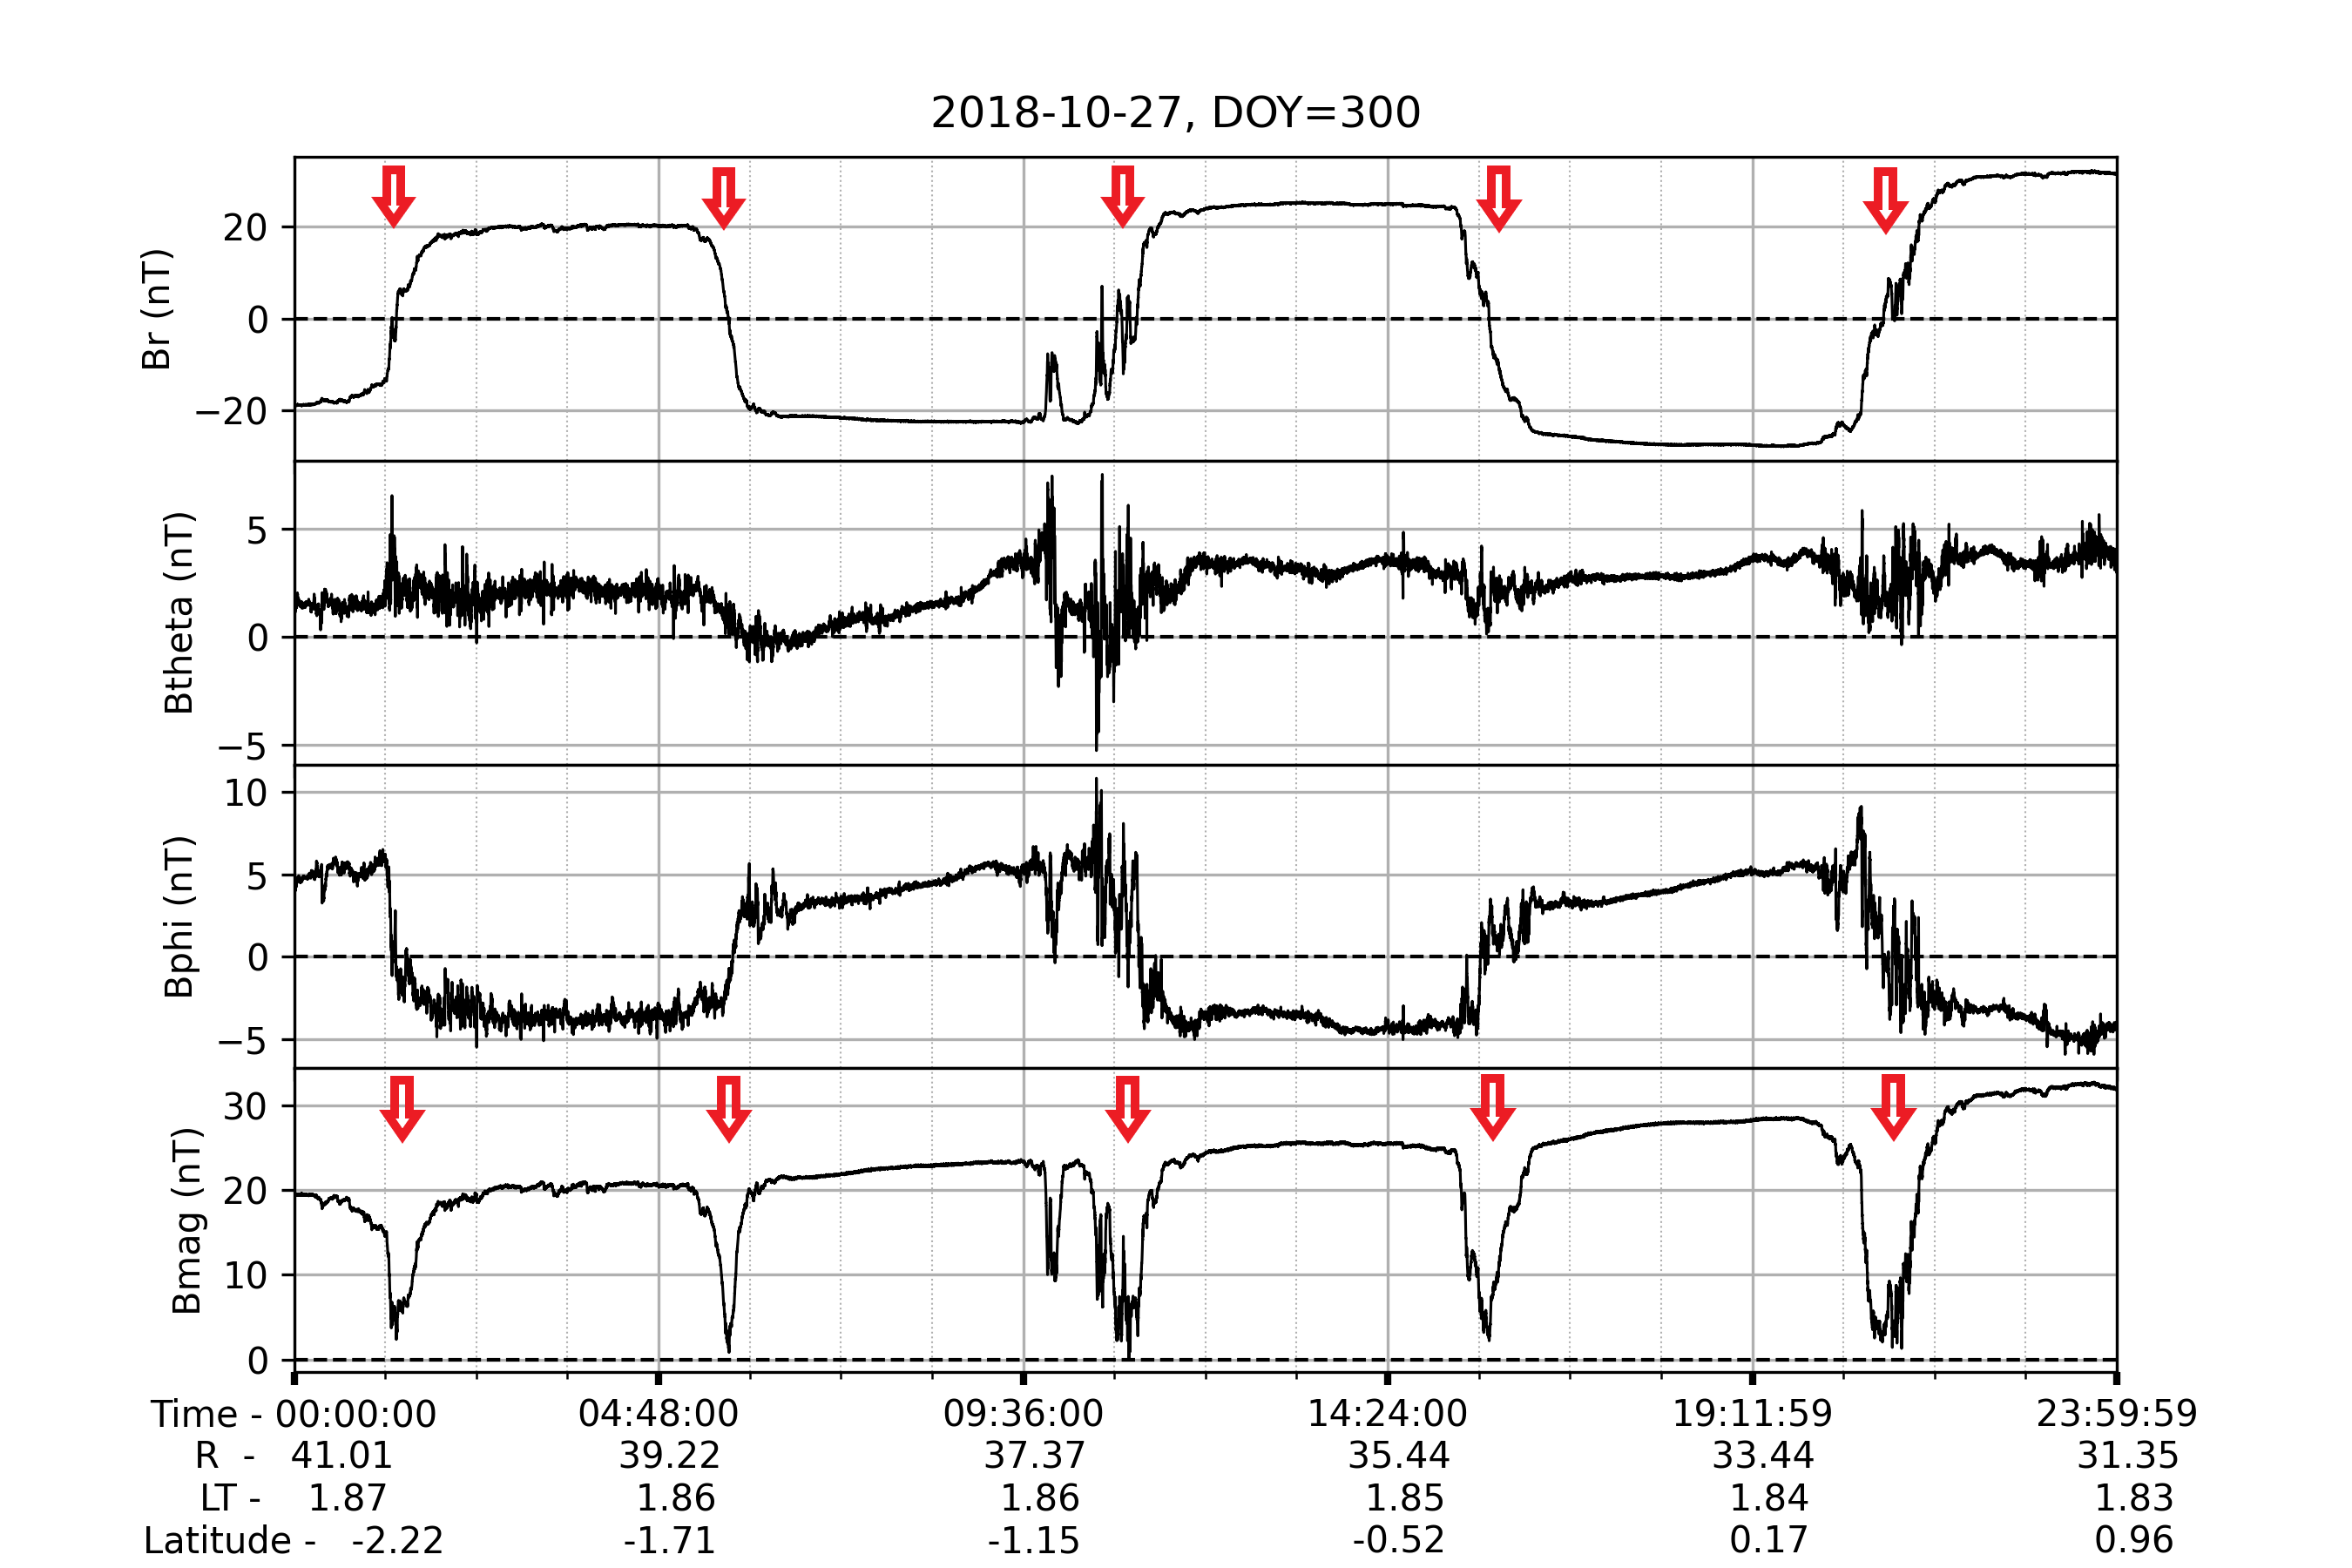
\includegraphics[width=\textwidth]{images6/Juno-currentsheet-observations.png}
    \caption{Magnetic field measurements taken by the Juno spacecraft in the JSS coordinate system ($B_r$, $B_\theta$, $B_\phi$, $|B|$). Juno crosses the current sheet twice every rotation period, as seen in the multiple reversals of $B_r$ separated by roughly $\sim$5 hours.}
    \label{fig:juno-current-sheet}
\end{figure}



Many empirical models have been put forward to account for the variation of the Jovian current sheet due to the non-axisymmetric internal field. Each model has a different set of parameters which are varied to minimize the error between the modeled current sheet location and that seen in-situ by the relevant spacecraft. Although they can be used to infer the location of the current sheet, these models do not provide any information about its strength. They can be categorized into two classes, which are discussed in the later sections. 

 After the flybys of Voyager 1 and 2, it was discovered that the current sheet crossings associated with a North-to-South rotation of the field were delayed compared to those associated with a South-to-North rotation of the field \cite{Behannon1981}. This led to the development of the concept called magnetotail `hinging', which proposed that instead of following the magnetic dipole equator at large radial distances, the maximum  extent of the current sheet was limited to certain heights in the $z$ direction. An example of current sheet hinging is shown in Figure \ref{fig:example-hinging}, where two current sheets are shown with and without the hinging parameter. Based on heuristic arguments that Jupiter's  magnetospheric interaction with the solar wind leads to the formation of a magnetotail, the current sheet models were modified to include the hinging phenomena. It was shown by \citeA{Behannon1981} that the inclusion of current sheet hinging decreases the RMS error between the modeled current sheet and the in-situ data, with which it was originally fitted.

In Chapters 4 and 5 we showed that the Jovian magnetosphere, which was previously assumed to be insensitive to changes in the upstream parameters, does respond to changes in the solar wind dynamic pressure and the interplanetary magnetic field in the form of changes to the magnetospheric configuration and strength of currents in the ionosphere. In this chapter, we discuss the influence of the solar wind dynamic pressure on the Jovian current sheet. Specifically, we seek to answer the following questions,

\begin{enumerate}
    \item Does solar wind dynamic pressure increase or decrease the hinging distance of the current sheet?
    \item Does solar wind dynamic pressure change the speed at which the current sheet wave propagates outward from the planet?
    \item What are the differences in the response of a magnetosphere to a forward shock in the solar wind when using an idealized versus a tilted dipole for the internal field?
\end{enumerate}


\subsection{Axial models of the current sheet}
Initial models assumed that the Jovian current sheet would be located in a plane corresponding to the magnetic equator of Jupiter, which would rotate at the planetary rotation period. The expected $z$ location of the current sheet at a given radial location in cylindrical coordinates $(\rho, \phi)$ could then be described simply as \cite{VanAllen1974EnergeticJupiter,Goertz1976TheMagnetosphere},

\begin{equation}
    z = -\rho \tan\theta_d \cos\left(\phi - \phi_d\right)
\end{equation}

Where $\theta_d$ is the tilt of the assumed planetary dipole field with respect to the rotation axis and $\phi_d$ provides the azimuthal location of the magnetic North pole. The rigid tilted plane model was found to be inaccurate at large distances, and the model was modified to limit the $z$ excursions of the current sheet at large radial distances. The first \emph{hinged} current sheet models \cite{Smith1974The10,Hill1974ConfigurationMagnetosphere} added a condition to limit these excursions beyond $\rho > a$, where $a$ is the hinging distance and is the only free parameter.
\begin{equation}
    z = \begin{cases}
    -\rho \tan\theta_d \cos\left(\phi - \phi_d\right), & \text{for } \rho \leq a\\
    -a \tan\theta_d \cos\left(\phi - \phi_d\right), & \text{for } \rho > a
    \end{cases}
\end{equation}

Or alternatively, using a $\tanh$ function, 
\begin{equation}
    z = -a \tanh\left(\frac{\rho}{a}\right) \tan\theta_d \cos\left(\phi - \phi_d\right)
\end{equation}

An improvement was suggested by \citeA{Kivelson1978ASheet} to add a phase delay to the current sheet location, proportional to the distance from the wave source and has the following functional form,
\begin{equation}
    \phi' = \phi_d - \frac{\Omega \left( \rho - \rho_0\right)}{U}
\end{equation}

Where $\Omega$ is the angular velocity of Jupiter, $U$ is the speed at which the wave travels and $\rho_0$ serves as the radial distance where the current sheet ceases to follow the rotating plane, beyond which all locations perceive a delay in the arrival of the current sheet. The expected current sheet location in the \citeA{Kivelson1978ASheet} model is then given by,
\begin{equation}
    z = \begin{cases}
    -\rho \tan\theta_d \cos\left(\phi - \phi_d\right), & \text{for } \rho < \rho_0\\
    -\rho \tan\theta_d \cos\left(\phi - \phi'\right),  & \text{for } \rho \geq \rho_0
    \end{cases}
    \label{eqn:kivelson1978}
\end{equation}

\citeA{Eviatar1976PlasmaMagnetosphere} introduced a similar model but limited the latitudinal extent of the oscillation beyond $\rho \geq \rho_0$,
\begin{equation}
    z = \begin{cases}
    -\rho \tan\theta_d \cos\left(\phi - \phi_d\right), & \text{for } \rho < \rho_0\\
    -a \tan\theta_d \cos\left(\phi - \phi'\right),  & \text{for } \rho \geq \rho_0
    \end{cases}
\end{equation}

Lastly, \citeA{Behannon1981} introduced another axial model which included the effects of wave propagation and current sheet hinging (Equation 11 in \citeA{Behannon1981}). However, they assume that the wave starts propagating from the origin $\rho_0=0$.
\begin{equation}
    z = -a \tanh\left(\frac{\rho}{a}\right) \tan\theta_d \cos\left(\phi - \phi_d + \frac{\Omega \rho}{U}\right)
    \label{eqn:behannon1981}
\end{equation}

\subsection{Non-axial models of the current sheet}
Axial models were found to fit the data poorly at large distances in the magnetotail, and it was suggested that the interaction of the magnetosphere with the solar wind may lead to a formation of a magnetotail, where the current sheet would take the form of a rocking plane instead of a rotating disk. However, the rocking plane model does not accurately represent the current sheet near the planet. \citeA{Behannon1981} suggested a hybrid model which follows the magnetic equator close to the planet and takes the form of a rocking plane at large distances (also called the Rocking Plane/Rotating Disk model or RP/RD).

\begin{equation}
    \phi' = \phi_d - \frac{\Omega \left(x - a\right)}{U}
\end{equation}
\begin{equation}
    z = x \sech \left( \frac{x}{a} \right) \cos\left(\phi - \phi' \right) + y \sin\left(\phi - \phi' \right)  
\end{equation}

Note that the above model follows a rotating disk near the planet where $\phi'=\phi_d$. The wave starts propagating at distance $a$ at a fixed speed $U$, which are the two parameters for this model. \citeA{Khurana1992a} extend the previous models by prescribing a variation in the wave propagation speed with radial distance as follows,

\begin{equation}
    v(\rho) = v_0 \coth \left(\frac{\rho}{\rho_0} \right)
\end{equation}
which leads to the following expressions for the phase delay and the current sheet location,
\begin{equation}
    \phi' = \phi_d - \Omega \int \frac{d\rho}{v(\rho)} = \phi_d - \frac{\Omega \rho}{v_0} \ln \cosh \left( \frac{\rho}{\rho_0} \right) 
\end{equation}
\begin{equation}
    z = -\rho \tan\theta_d \cdot \frac{x_0}{x} \tanh\left(\frac{x}{x_0} \right) \cos\left( \phi - \phi'\right) 
    \label{eqn:khurana1992}
\end{equation}
The \citeA{Khurana1992a} model has three parameters $(v_0, \rho_0, x_0)$ representing the asymptotic wave propagation speed, radial location of outflow, and the hinging point along the X-axis to account for the interaction with the solar wind. \citeA{Khurana2005} updated the model to account for local time asymmetries and solar wind angle of attack, but the generalization increases the number of parameters in the model. 

\begin{figure}
    \centering
    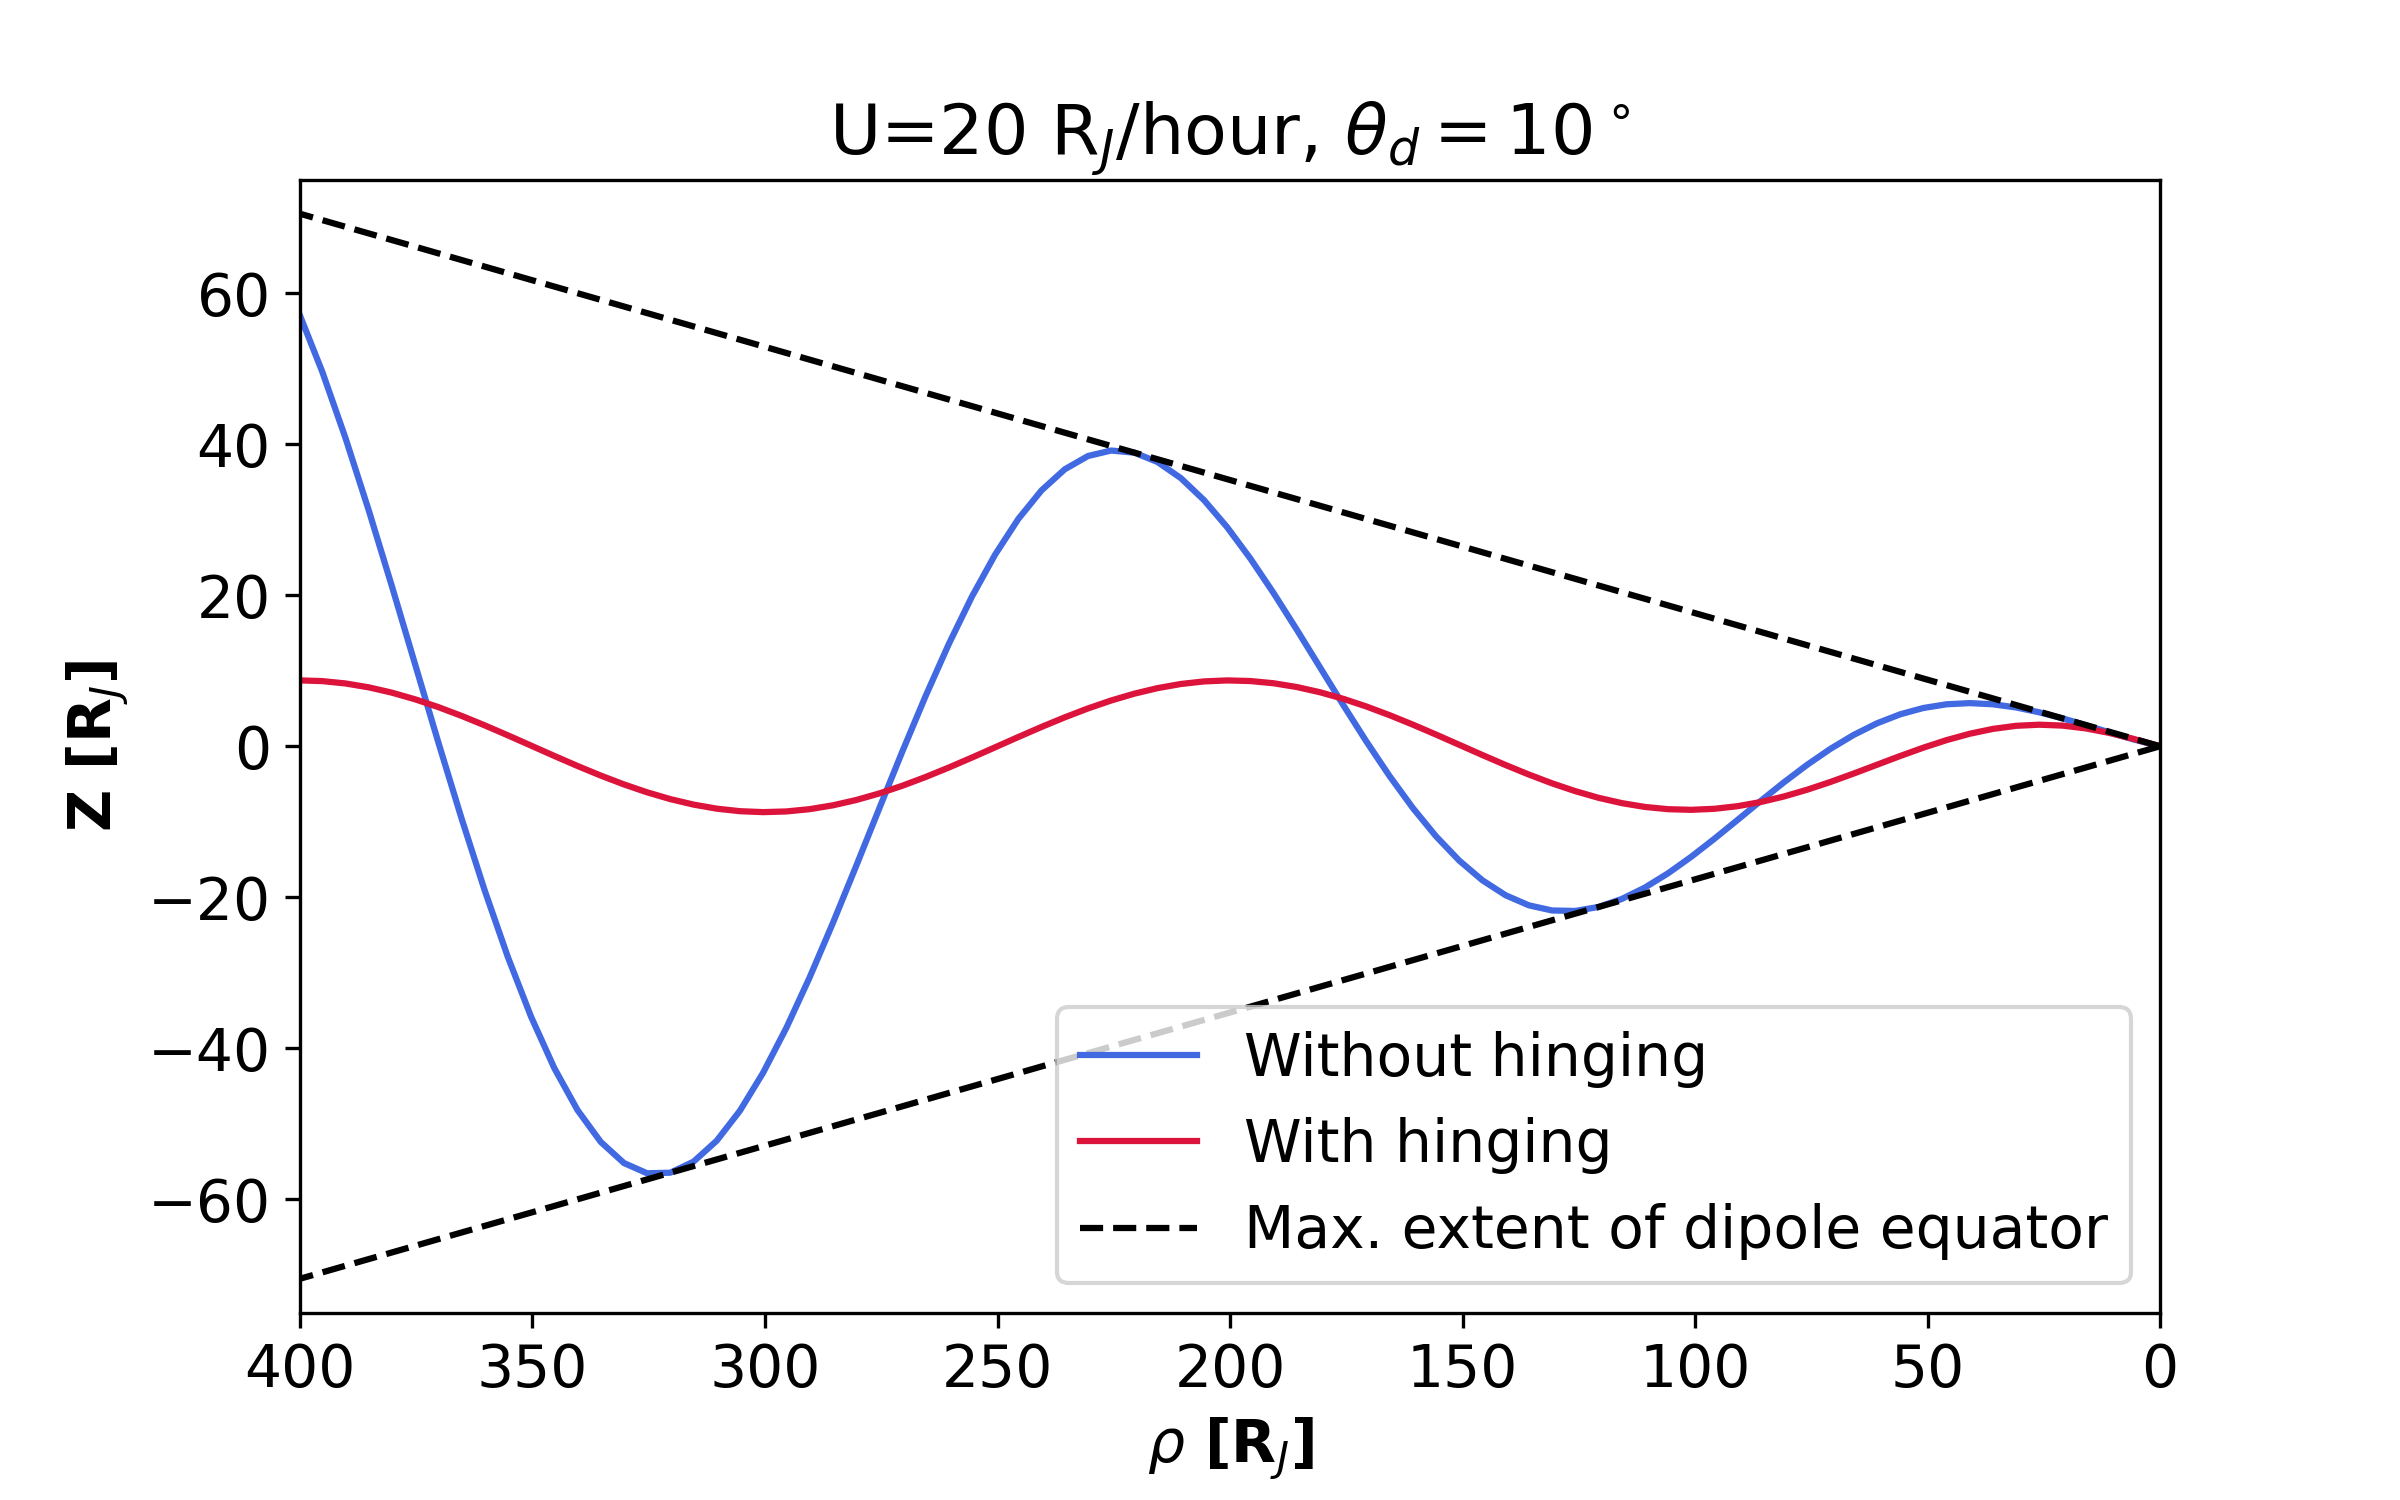
\includegraphics[width=0.8\textwidth]{images6/example-hinging.png}
    \caption{Examples of the Jovian current sheet locations for two different models. The \protect\citeA{Kivelson1978ASheet} model does not account for hinging of the current sheet and hence has larger excursions with increasing distance from the planet. The \protect\citeA{Behannon1981} model includes current sheet hinging, which limits the oscillations beyond a certain radial distance.}
    \label{fig:example-hinging}
\end{figure}

\section{Methodology}

\subsection{MHD simulations with a tilted dipole}
To simulate the modulation of the Jovian current sheet, we modify the internal magnetic field of Jupiter to take the form of a dipole tilted 10$^\circ$ with respect to the spin axis and rotates around it at the planetary rotation period (10 hours). The simulations are performed in the GSE coordinate system. In the simulations shown in Chapters 3 and 4, we used a spherical grid. Through our tests, we found that a spherical grid is not ideal when simulating a time-varying magnetosphere, where density and magnetic structures frequently cross the polar regions of the planet where grid cells are small and have a large aspect ratio. To circumvent this problem, we use a cartesian grid in the simulations performed for this study. The cartesian grid contains roughly 19 million cells, with the lowest grid resolution of 0.125 $R_J$ present near the planet and the Io torus. 

Different upstream conditions are introduced to evaluate the response of the current sheet to varying solar wind dynamic pressure. The properties of the solar wind used for the three runs are tabulated in Table \ref{tab:sw-conditions-chp6}.

\begin{table}
    \centering
    \begin{tabular}{c|c|c|c|c|c}

    Run  &$B$  &$u$  &$\rho$     &$T$  &$p_d$\\
         &nT   &km/s &amu/cm$^3$ &K    &nPa\\
    \hline
    1    &0.31  &322.04  &0.062  &4.3E2  &0.011\\
    2    &1.00  &400.00  &0.200  &2.0E5  &0.053\\
    3    &2.82  &532.46  &0.564  &8.8E5  &0.267\\

    \end{tabular}
    \caption{Solar wind magnetic field strength, speed, density, temperature and dynamic pressure used in the present study. The variables are prescribed at the upstream boundary of the simulation at $X=192$ $R_J$. The interplanetary magnetic field is oriented along the negative $Z$ direction.}
    \label{tab:sw-conditions-chp6}
\end{table}

\subsection{Estimating the current sheet parameters within the MHD model}
The current sheet location in our model varies with radial distance and dipole phase. A direct comparison between the current sheet location in the MHD model and the various empirical functions shows a poor fit, as small differences in phase can lead to large differences in the final current sheet location. Moreover, the empirical models have been observed to perform well only for the in-situ data to which they were originally fitted \cite{Khurana1992a, Behannon1981}. For a more accurate comparison, we use the functional form for the various empirical models to find the set of parameters e.g. hinging distance, wave propagation speed, etc. which reproduce best the output seen in the MHD simulations.

We consider three models with relatively simple functional forms,
\begin{enumerate}
    \item The \citeA{Kivelson1978ASheet} model described by Equation \ref{eqn:kivelson1978} with two parameters - $U$ and $\rho_0$, corresponding to the speed of wave propagation and the radial location where the current sheet wave starts to propagate. 
    \item The \citeA{Behannon1981} model described by Equation \ref{eqn:behannon1981} with two parameters - $U$ and $a_0$, corresponding to the speed of wave propagation and the radial location where hinging is introduced.
    \item The \citeA{Khurana1992a} model described by Equation \ref{eqn:khurana1992} with three parameters - $v_0$, $x_0$ and $\rho_0$, corresponding to the asymptotic speed of wave propagation, the characteristic hinging distance in the $x$ direction and the radial location where the wave outflow commences. 
\end{enumerate}

The location of the current sheet is extracted in the noon-midnight meridian (00 LT) by identifying the locus of points located between $x=[-100, -4] R_J$ and $z=[-30, 30] R_J$ where  $B_r=0$. A current sheet model is then fitted to the extracted current sheet height $z_\text{MHD}$ at a given radial location $\rho$ by finding the set of parameters $\boldsymbol\theta$ that minimizes the square of the residual $\mathcal{R}$, which is normalized to the standard deviation of the current sheet location in the MHD model ($z_\text{MHD}$),

\begin{equation}
    \mathcal{R} = \frac{1}{\sigma(z_\text{MHD})} \sum_i^N \left[ z_\text{MHD}(\rho) - z_\text{fit} (\rho, \boldsymbol\theta) \right]_i^2
\end{equation}

The Levenberg-Marquardt iterative algorithm is used to perform the non-linear minimization for all models except the \cite{Kivelson1978ASheet} form, for which the more robust Nelder-Mead algorithm is used. We repeat the above procedure for all simulation data files separated by an interval of 30 minutes, giving us 200 data points within a 100 hour interval for each model. Although we limit our analysis to regions in the $y=0$ plane and $x < -4 R_J$ (nightside magnetotail), we effectively sample different phases of the current sheet due to the rotation of the dipole every 10 hours.

\begin{figure}
    \centering
    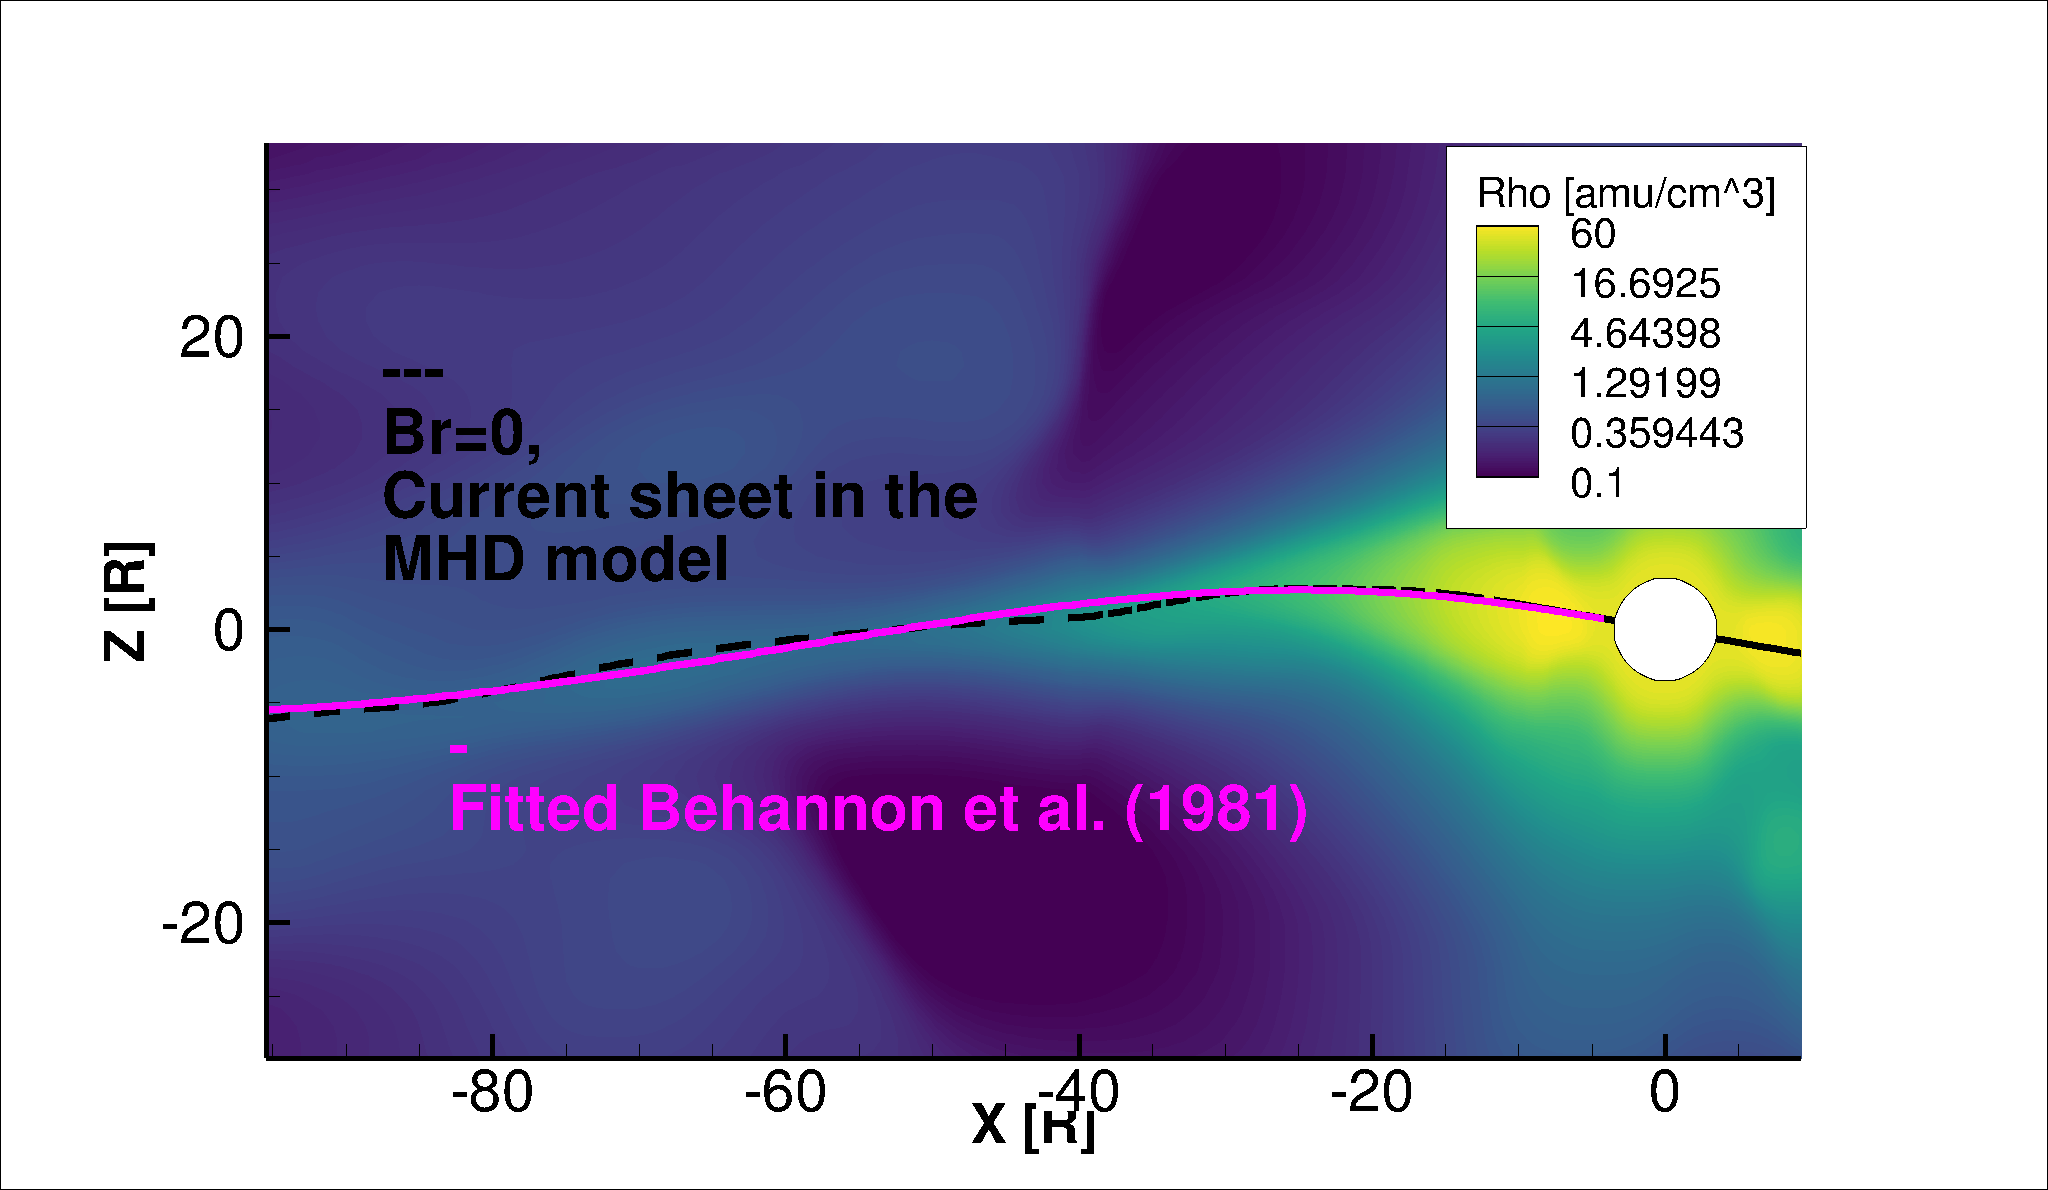
\includegraphics[width=\textwidth]{images6/CurrentSheet_fitted.png}
    \caption{Caption}
    \label{fig:example-fitcurrentsheet}
\end{figure}

Figure \ref{fig:example-fitcurrentsheet} shows the result of fitting the \citeA{Behannon1981} model for the current sheet to that observed at that instance in the MHD simulations. In this instance, the wave velocity $U$ and the hinging distance $a_0$ are estimated to be 20.8 $R_J$/hour (413.0 km/s) and 32.4 $R_J$ respectively. 

\section{Results}

We investigate the response of the current sheet parameters to the solar wind dynamic pressure by introducing three different upstream cases which are described in Table 1. 

\subsection{The Kivelson et al. (1978) form}

\begin{figure}
    \centering
    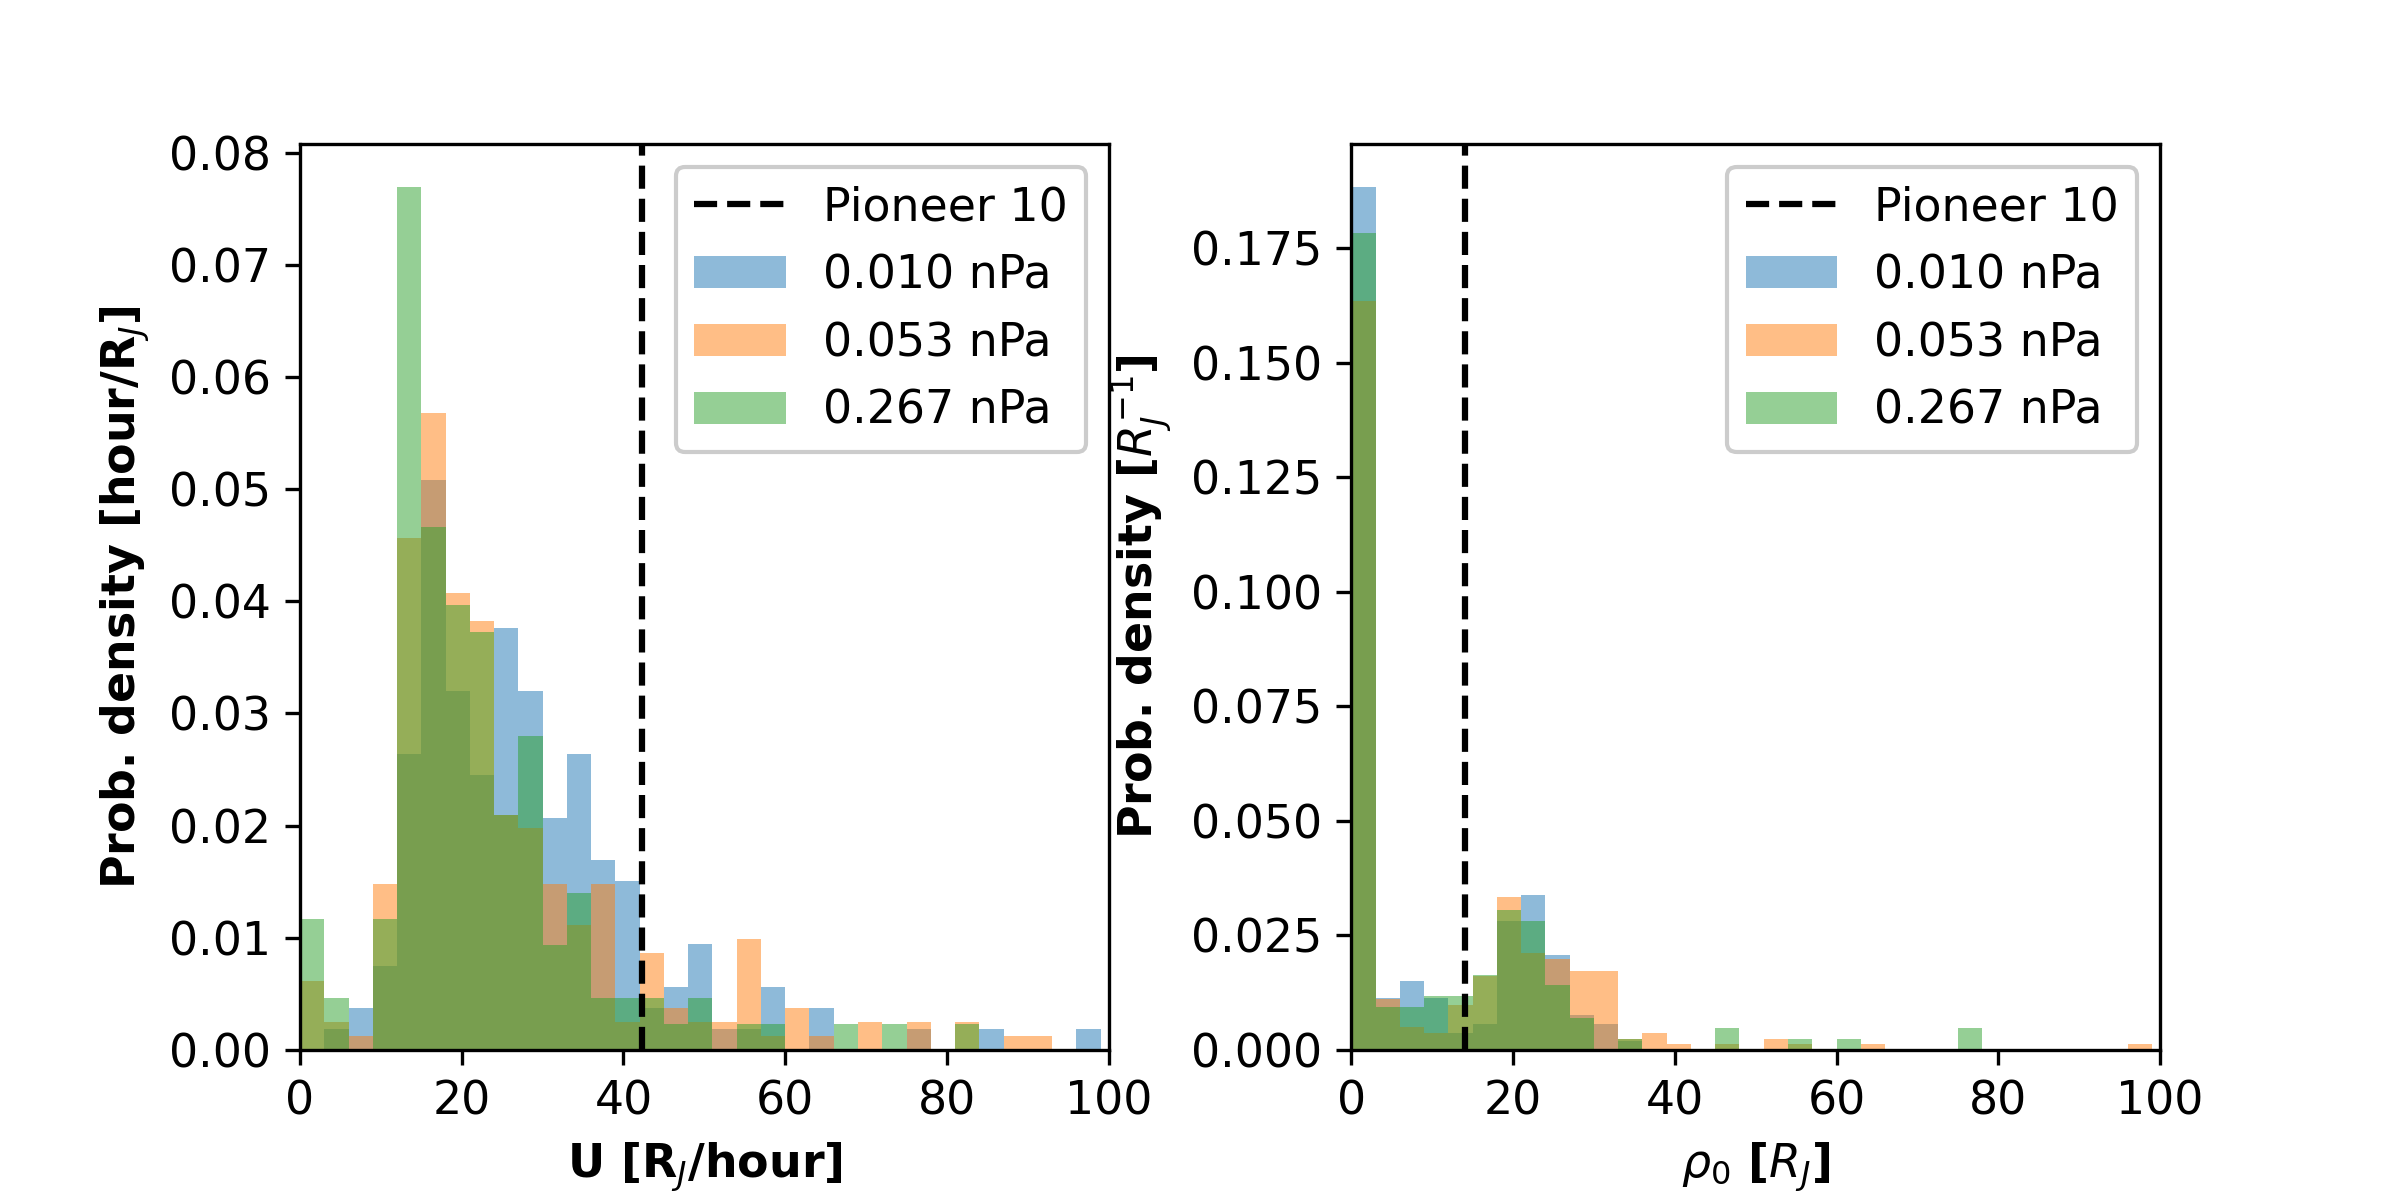
\includegraphics[width=\textwidth]{images6/comparison_highdynP_kivelson.png}
    \caption{Caption}
    \label{fig:comparison-hist-kivelson}
\end{figure}

Fitting Equation \ref{eqn:kivelson1978} to the current sheet extracted from the simulation yield two parameters - the wave propagation speed $U$ and the radial location where wave propagation begins $\rho_0$. The parameters which fit best the simulation results are plotted in a histogram in Figure 
\ref{fig:comparison-hist-kivelson} for the three dynamic pressures. The number of simulation times for which a good fit is obtained varies for the different runs. For a meaningful comparison, we normalize the histogram such that the area under each histogram sums to unity. 

The histograms for the wave propagation speed show a considerable spread of possible values, ranging from $\sim$10 $R_J$/hour (198.6 km/s) to $\sim60 R_J$/hour (1191.5 km/s), though the distribution is skewed to lower values. With increasing dynamic pressure, the skew in the distribution shifts more to lower values, indicating that the wave propagation speed is lower during intervals when the solar wind dynamic pressure is high. 

On the other hand, the distribution of $\rho_0$ in the MHD model overwhelmingly favours low values of $\rho_0$ and is insensitive to change in the solar wind dynamic pressure. Low $\rho_0$ values imply that the current sheet wave begins propagating at a finite speed very close to the planet. 

\subsection{The Behannon et al. (1981) form}
\begin{figure}
    \centering
    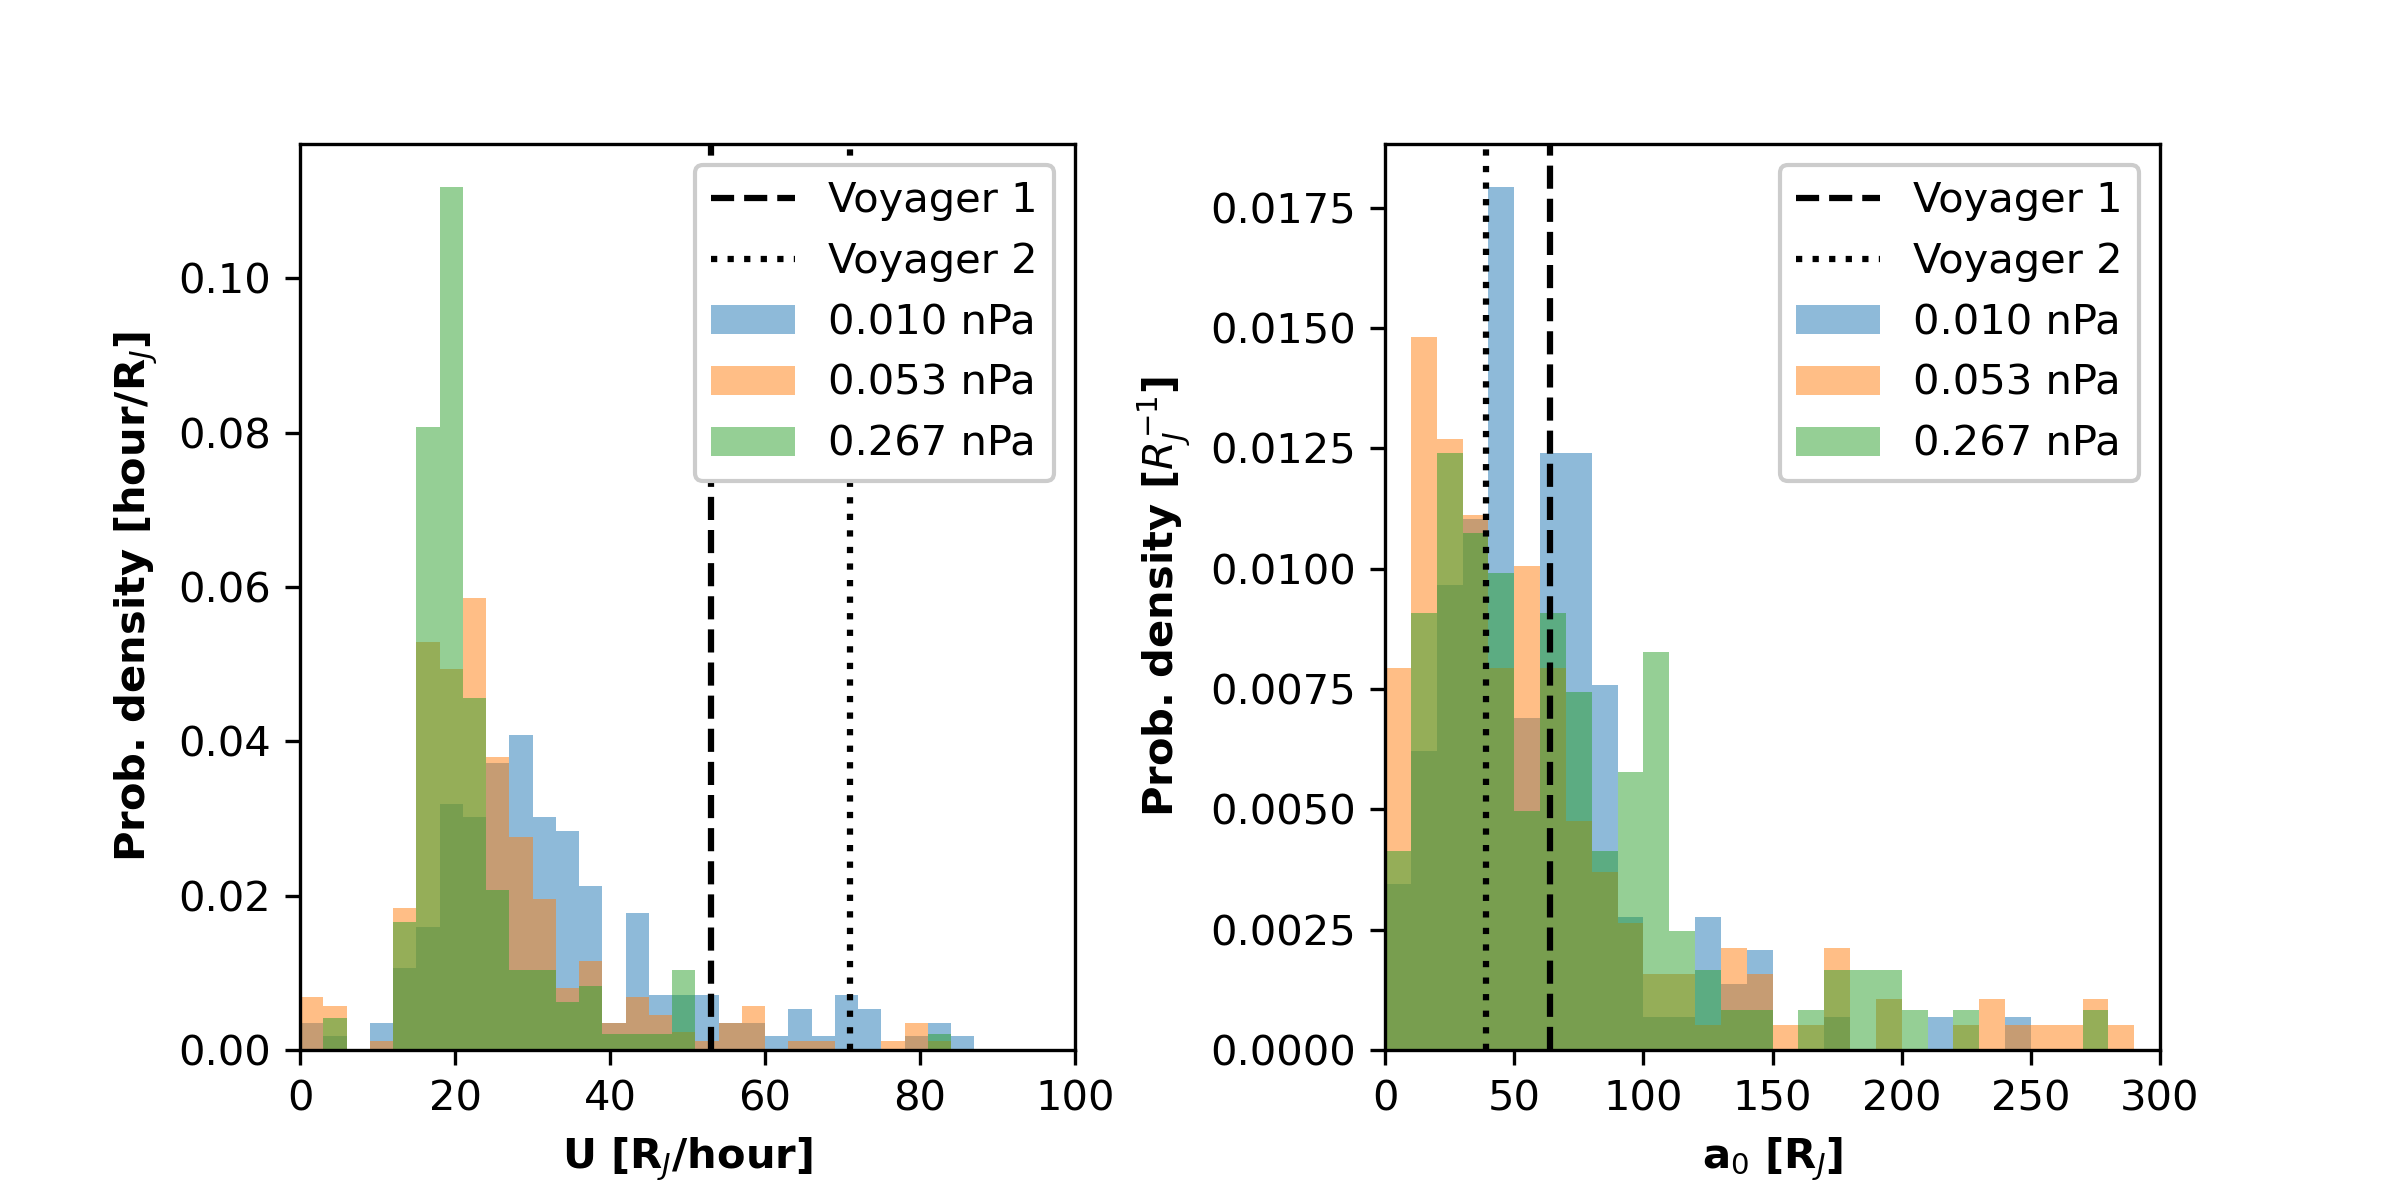
\includegraphics[width=\textwidth]{images6/comparison_highdynP_behannon.png}
    \caption{Caption}
    \label{fig:comparison-hist-behannon}
\end{figure}

This model described by Equation \ref{eqn:behannon1981} contains two parameters - the wave propagation speed $U$ and the distance $a_0$ beyond which the current sheet is \emph{hinged}, i.e. its maximum extent in the $z$ direction is limited. As before, we show the normalized histograms of these parameters in Figure \ref{fig:comparison-hist-behannon}. 

Similar to the result obtained when using the \citeA{Kivelson1978ASheet} form, the speed of the current sheet wave varies between 15 to 50 $R_J$/hour. For lower solar wind dynamic pressure (0.010 nPa), the mean of the distribution is located at 30 $R_J$/hour and shift to lower values for higher solar wind dynamic pressure. This result is consistent with the previous model and supports the conclusion that increasing solar wind dynamic pressure slows the propagation of the current sheet wave. 

The hinging parameter $a_0$ also exhibits large variations, with most values ranging between 0 to 100 $R_J$. The mean $a_0$ is seen to be anti-correlated with solar wind dynamic pressure. 
 
\begin{figure}
    \centering
    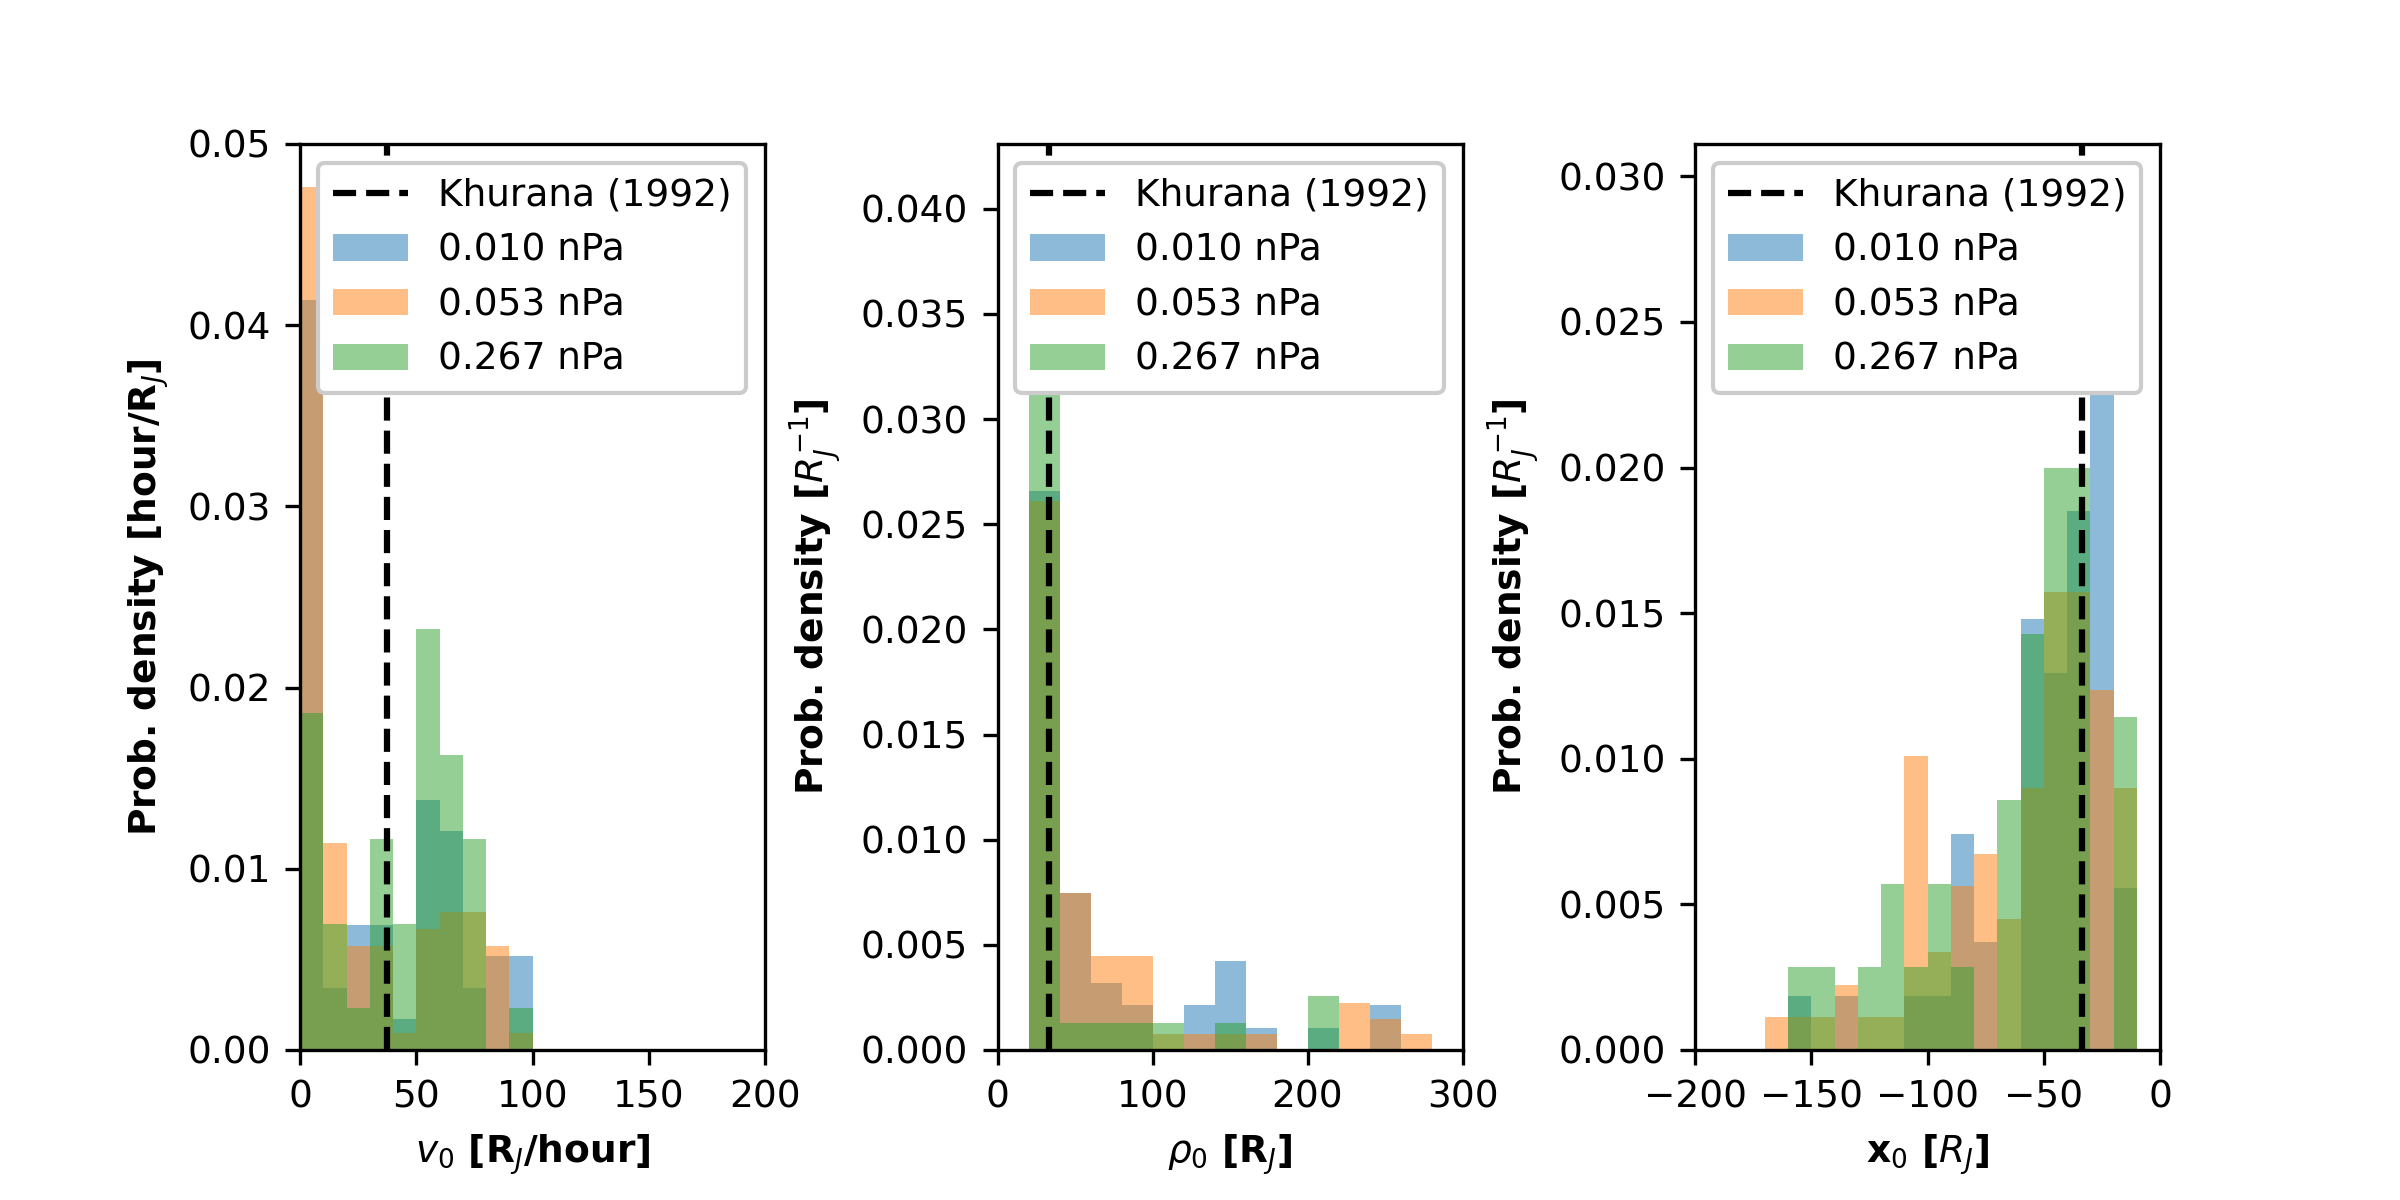
\includegraphics[width=\textwidth]{images6/comparison_highdynP_khurana.png}
    \caption{Caption}
    \label{fig:comparison-hist-khurana}
\end{figure}


\section{Discussion}
\section{Summary}